\documentclass[a4paper,12pt,twoside]{article}
\usepackage{geometry}
\usepackage{csvsimple}
\usepackage{graphicx}
\geometry{a4paper, margin=2cm}
\usepackage{xstring}
\usepackage[T1]{fontenc}
\usepackage{xcolor}
\usepackage{subcaption}
\usepackage{float}
\usepackage{charter}
\usepackage{url}
\usepackage{hyperref}
\setlength\parindent{0pt}

\title{\textbf{The HiWi's Guide to the \\Booklet Builder}}
\date{Version 3, February 2025}
\author{maja.lecher@uni-bayreuth.de}

\begin{document}

\maketitle
\newpage

Welcome to the Booklet Builder Guide! It is here to make your life easier.

\section{What is LaTeX and why bother using it?}
This booklet builder is written in \LaTeX. \LaTeX is a high-quality typesetting system that is routinely used for scientific documents, as well as almost any form of publishing. 

Its power lies not only in its ability to consistently output files in exactly the format you envisioned (no more of that figures-emigrating-to-Hawaii-when-adding-a-single-letter-somewhere!), but also in its capacity to automatise tedious, repetitive tasks like building a species list.

If you’re not used to the modular nature of \LaTeX, the many output files with obscure endings may look a bit daunting at first — but don’t worry, it’s easier than it seems and you’ll get the hang of it in no time.

If all goes well, you will never have to touch the source code for the booklet builder beyond changing the occasional file path anyway, but in case things do go wrong, need tweaking, or you’re bored, I have included a crash course in section \ref{sec:crashcourse}.

\section{What do I need on my computer?} \label{ch:computer}
\begin{enumerate}
    \item A \textcolor{red}{\textbf{LaTeX editor}} \\
        \LaTeX is a markup language, so you could technically write your source code in any text editor, but in order for your code to compile and turn into a shiny pdf document, you need a dedicated \LaTeX editor.
        \begin{itemize}
            \item For smaller files (with, say, 50 different species), it should be sufficient to use an online \LaTeX editor like \textcolor{orange}{Overleaf} (\url{https://www.overleaf.com/}). Overleaf has the advantage of being free (with some limitations) and collaborative, allowing multiple people to work on the same project at once, and you don’t need to install anything. The downside is that once your file exceeds a certain size or you want more than two collaborators to work on the project simultaneously, you would need to upgrade to a paid version. The University of Bayreuth does not, to my knowledge, provide free premium accounts. 
            
            \item  If the file becomes too large or you want to work on your project locally, you can move to one of the many editors capable of compiling \LaTeX  code. I personally recommend \textcolor{orange}{TeXMaker}, which is a dedicated \LaTeX   editor. TeXMaker is open source and cross-platform, meaning that Windows, Linux, and MaC OS users alike should be able to work with it. If you’re already working with programming languages like R or Python and already have a preferred integrated development environment (like \textcolor{orange}{Visual Studio} or \textcolor{orange}{Sublime}), you can also use that. This guide will include screenshots of both TeXMaker and Overleaf as examples. 
            In order for your editor to interpret \LaTeX \ code, you also need to install \textcolor{red}{TeX Live}. This isn't complicated, but unfortunately takes a while (up to four hours) due to its large size. You can find a list of installation/good instruction links below:
            \begin{itemize}
                \item Step-by-step instructions (by Uni Regensburg): \url{https://www.uni-regensburg.de/assets/physik/fakultaet/Studium/LaTeX/Anleitung\_Installation\_LaTeX\_01.pdf}
                \item TeX Live: \url{https://www.tug.org/texlive/}
                \item TeXMaker: \url{https://www.xm1math.net/texmaker/download.html}
            \end{itemize}.
        \end{itemize}
    \item \textbf{Logos}
        To make the booklet pretty, the title page includes logos of the University of Bayreuth and of the faculty. These files are stored in a folder called \textcolor{red}{\texttt{Logos}}. It contains the following files:
        \begin{itemize}
            \item \textcolor{red}{\texttt{biogeo.jpg}}
            \item \textcolor{red}{\texttt{dist\_eco.jpg}}
            \item \textcolor{red}{\texttt{GCE-Logo.jpg}}
            \item \textcolor{red}{\texttt{Uni\_Bayreuth.jpg}}
        \end{itemize}
    \item \textbf{Files}\\ 
        \LaTeX is modular, meaning that different tasks (like making the title page or listing all species) can be dealt with in separate files. This approach makes it easy to only change what needs to be changed. The master file, typically titled \texttt{main.tex}, generally both contains main body of your document and deals with arranging the content from other files with specialised tasks. These files are referenced by their file path and filename, therefore it is important to make sure that you \textbf {do not accidentally change the file names}, and that \textbf{all files remain in the same folder}. \\

        \fbox{ \begin{minipage}{35em}
            \textbf{NOTE}: A word on \texttt{.csv} files and the importance of checking raw text files.\\            
            \raggedright The ending \texttt{.csv} is short for \emph{comma-separated value}. These types of files can be opened using spreadsheet programs like Excel or LibreOffice Calc for easy viewing, but internally, they are only simple lines of text without any formatting. Spreadsheet programs recognise certain characters in these text files, usually commas, as cell boundaries, and display them as such — for example, the line \\ 
            {\centering \texttt{column A, column B, column C}\par }
            %\centering {\texttt{column A, column B, column C}} \\ 
           \raggedright would be displayed as \hfill \\ 
            {\centering \texttt{| column A | column B | column C |}\par }
            
            in a spreadsheet program. While commas are typically the default setting for boundaries, it is possible to use a different character like a semicolon. This is the case for the Booklet Builder in order to make it possible to add notes that include commas in sentences. The \LaTeX files for the Booklet Builder are likewise explicitly written to interpret semicolons, not commas, as entry separators.
            
            This means that \textbf{if you choose to open any of the content files with a .csv ending using a spreadsheet program} for easy viewing and editing, please be aware that when you open or close it, the program may ask you about “separator options”. \textbf{Make sure you choose “separated by semicolon”}, otherwise any commas in the text will be re-interpreted as cell boundaries by the program, the spreadsheet may re-encode all semicolons as commas, and as a result, the \LaTeX files will not be able to properly interpret your input files.
            
            It is an easy mistake to undo, but can be a hassle. If you want to circumvent this issue altogether, troubleshoot, or double check, you can also choose to open .csv files in simple text editors like Microsoft Notepad or Kate, although it’s less pretty than viewing it as a spreadsheet.
        
            Spreadsheets may also have trouble displaying special characters like German Umlaute. If this is the case, this should only be a problem when viewing in the spreadsheet program itself. As long as you make sure the character encoding is "Western Europe (ISO-8859-15/EURO)", it will not be an issue in the final document output. 
           \end{minipage}
        }

    \begin{itemize}
        \item \textbf{Content files} \\
            These are the files meant to be changed by you.
            \begin{itemize}
                \item \textcolor{red}{\texttt{booklet\_title.csv}} \\This file includes the title of your booklet, location, version, date, author, sources, etc. (\textbf{Note the file ending! The content file is a \texttt{.csv} file. If the file ending is \texttt{.tex}, you are looking at the typesetting file discussed below)}.
                \item \textcolor{red}{\texttt{species\_list.csv}} \\This file is the heart and soul of the booklet! It includes a list of the species, genus, family, author, synonyms, German names, comments, and the file paths for the identification pictures.
            \end{itemize}
        \item \textbf{Typesetting files} \\
            These files compile and typeset all the information stored in the content files. They are written such that you should not need to touch them, unless you specifically want to change the typesetting, the file path of the content files, or need to debug something. \\
            
            \begin{itemize}
                \item \textcolor{red}{\texttt{booklet\_title.tex}} \\ Formats the title page of the booklet. 
                \item \textcolor{red}{\texttt{main.tex}} \\ Formats the main body of the text and outputs the final PDF file.
            \end{itemize}
    \end{itemize}

    \item Empty folder named \textcolor{red}{\texttt{Images}} \\
        Each species in the booklet typically includes two identification images. These are often sourced from Flora Helvetica (https://www.infoflora.ch/en/) and Rothmaler. You will need to download these yourself (depending on the content of the booklet), and make sure you store them in a folder called "Images", as the filepath in the .tex files specifically references this folder.
    \end{enumerate}

    And you're all set to start working! The step-by-step workflow is explained in the next section.

    \newpage

    \section{Workflow}
        \subsection{Changing the booklet title} \label{ch:title}
            \begin{itemize}
                \item Open \texttt{booklet\_title.csv}. If you open it using a spreadsheet program like Excel or LibreOffice Calc, it should look something like fig. \ref{fig:booklet_title_csv}. If, instead, you're using a plain text editor, it should look like fig. \ref{fig:booklet_title_csv_plain}. If it doesn't, please refer to the note about \texttt{.csv} files in section \ref{ch:computer}.

                    \begin{figure}[h]
                      \centering
                      \begin{subfigure}[b]{0.9\textwidth}
                        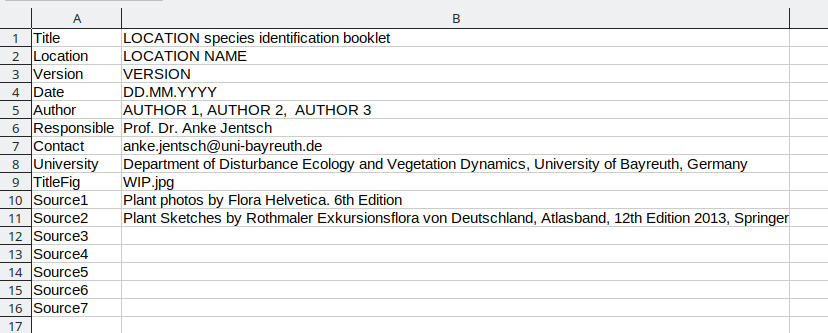
\includegraphics[width=\textwidth]{booklet_title_csv.png}
                        \caption{Spreadsheet}
                        \label{fig:booklet_title_csv}
                      \end{subfigure}
                      \hfill
                      \begin{subfigure}[b]{0.9\textwidth}
                        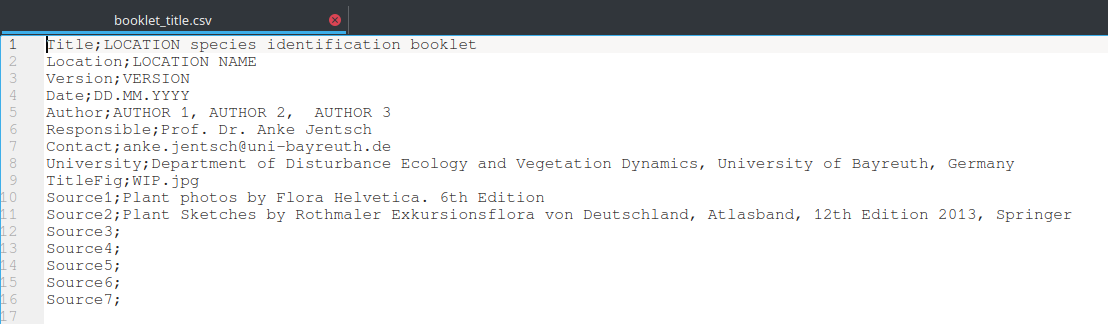
\includegraphics[width=\textwidth]{booklet_title_csv_plain.png}
                        \caption{Plain text}
                        \label{fig:booklet_title_csv_plain}
                      \end{subfigure}
                      \caption{booklet\_title.csv}
                      \label{fig:figure}
                    \end{figure}

                \item Change the \textcolor{red}{content in column B} (or, equivalently, anything after the semicolon in plain text) as needed. All fields are optional, if a line isn't necessary, just leave it blank. \textbf{Do not delete any rows!}
                \item Save and close the file. If asked, \textbf{make sure you save it as a \texttt{.csv} file with "semicolon" as separator, and as a \texttt{.csv} file. Don't let your spreadsheet program change the file type to \texttt{.ods} or \texttt{.xls}!}. Also make sure the file is encoded in as "Western Europe (ISO-8859-15/EURO)", otherwise German Umlaute (ä, ö, ü, ß) will not compile properly. The encoding option typically pops up in the same window as the separator options when you open or save the file.
            \end{itemize}
            
        \newpage
        \subsection{Creating a species list}
            \begin{itemize}
                \item Open \texttt{species\_list.csv}. Same \texttt{.csv} caveats as outlined in section \ref{ch:title} apply.
                \item For each species, you can now add the \textcolor{red}{name, author, any synonyms, genus, family, its local name}, and, if you wish, \textcolor{red}{comments}. All fields are optional and can be left blank. \\Important notes: \begin{itemize}
                    \item Make sure not to change the column names! The \LaTeX script explicitly refers to these names.
                    \item If you want to include the character "\&" (e.g. for multiple authors), \textbf{add a backslash in front of the "\&"}, i.e. "$\backslash$\&". LaTeX will otherwise interpret it as an internal command and output gibberish.
                \end{itemize}
                \item The columns \texttt{FileNamePhoto} and \texttt{FileNameID} are explained in section \ref{ch:filenamephoto}
                \item Sort the species list according to how you wish it to be displayed in the booklet (i.e. if you want them sorted alphabetically by name, select that column and sort accordingly. If you want to also sort by Family, sort by that column.)
                \end{itemize}
                                          
        \subsection{Downloading ID images} \label{ch:filenamephoto}
            Each species is typically shown using two images: one photo, and one drawing. Each booklet entry therefore has space for two figures.
            \begin{itemize}
                \item Download your ID pictures. This can be done, for example, via screenshots of the digital Rothmaler, or simply by saving photos from the Flora Helvetica webpage.
                \item Save all pictures in the \texttt{Images} folder. \textbf{Make sure to name each file clearly and without spaces}, e.g. \texttt{Acer\_pseudoplatanus\_photo.jpg} and \texttt{Acer\_pseudoplatanus\_ID.jpg} for the photo and the ID picture, respectively.
                \item Add the file names to the \texttt{species\_list.csv} file (see also fig. \ref{fig:example}). \textbf{It is not necessary to include the full file path as long as each image is stored in the \texttt{Images} folder.}
                \item Save and close the \texttt{species\_list.csv} file. 
            \end{itemize}
        The finished species list should look something like fig. \ref{fig:example}
                
            \begin{figure}[h]
                \centering
                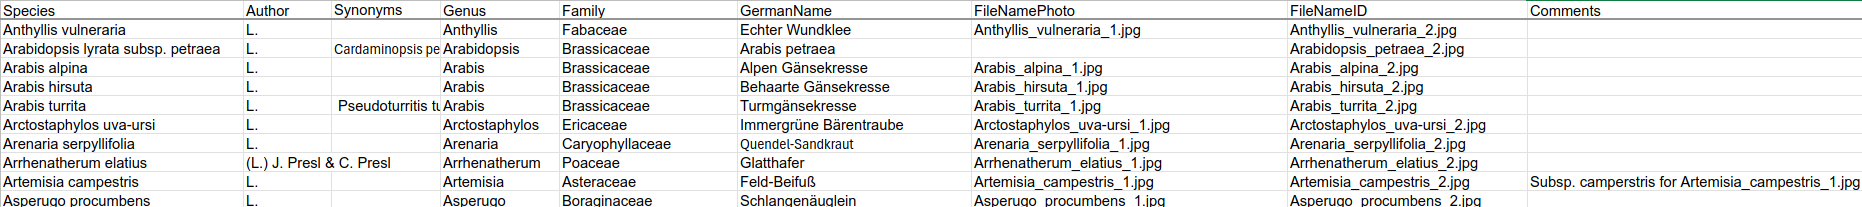
\includegraphics[width=1\linewidth]{example.png}
                \caption{species\_list.csv}
                \label{fig:example}
            \end{figure}
            
        \subsection{Compile the booklet}
            As mentioned in section \ref{ch:computer}, it is up to you whether you want to use something like Overleaf or work locally. The former may be easier to deal with at the beginning. 
            
        \subsubsection{If you're working with Overleaf} 
            
            \begin{itemize}
                \item Compress all Booklet Builder files into a \texttt{.zip} file. On windows, this is easily done by selecting all files in your file manager, right-clicking it, and selecting \texttt{Send to} $\rightarrow$ \texttt{Compressed (zipped) folder}. On MacOS and Linux, just select \texttt{Compress}. Your compressed folder should include
                    \begin{itemize}
                        \item The \texttt{Images} folder containing your ID pictures
                        \item The \texttt{Logos} folder containing the university logos
                        \item The typesetting file \texttt{main.tex}
                        \item The typesetting file \texttt{booklet\_title.tex} 
                        \item The content file \texttt{booklet\_title.csv}
                        \item The content file \texttt{species\_list.csv}.
                    \end{itemize}
                \item Go to https://www.overleaf.com/ and set up an account.
                \item In Overleaf: open a new project using the big green \texttt{New Project} button at the top left. Select \texttt{Upload Project}.
                \item Select or drag your newly created \texttt{.zip} folder into the popup window.
            \end{itemize}
        And that's it! Your project should automatically compile and output a PDF. Your file will include a table of contents at the beginning, which will update automatically if you change anything in your species list. You can download your PDF using the \texttt{Download PDF} icon next to the green \texttt{Recompile} button on the upper right.
        
        \subsubsection{If you're working locally}    
            \begin{itemize}
                \item Open the file \texttt{main.tex} in TeXMaker (either by starting up TeXMaker and selecting File > Open > [your filepath], or by right-clicking \texttt{main.tex} in your file browser, and selecting "Open with TeXMaker")
                \item In TeXMaker: Press the button next to "Quick Build", wait a few seconds for the compilation to finish, and pressing the button next to "View PDF" (see also fig. \ref{fig:texmaker} below). \textbf{Note: make sure that \texttt{main.tex} is located in the same folder as the remaining files and folders!}
                
                \begin{figure}[h]
                    \centering
                    
\includegraphics[width=0.8\linewidth]{TeXMaker.png}
                    \label{fig:texmaker}
                    \caption{TeXMaker}
                \end{figure}
            \end{itemize}
            And that's it! The folder should now automatically contain a pdf file named \texttt{main.pdf}. This is your finished file, feel free to re-name it.
            

    \subsection{Workarounds}
        Now all the tedious leg work is done and you have the backbone of your booklet, you may want to tweak little things, insert exceptions, or add a special page that only your project needs. While this can't be done using the BookletBuilder directly (imagine how bloated everything would get if every eventuality was coded in), there are workarounds that should allow you to do everything you need. 
        If something isn't listed below: get creative!

        \subsubsection{I can't find an ID image and need to describe my species using words}
            This is easy: write your description in a text editor of your choice, take a screenshot, and just use that picture instead of the ID photo. \\

        \emph{WORK IN PROGRESS}
        %\subsubsection{I want to add a page/an element in }
        %    Create the page you want and splice it into your document
        
    
        \section{Troubleshooting}
            \emph{Will update after feedback}. 

        \section{LaTeX crash course} 
        \label{sec:crashcourse}
        \emph{WORK IN PROGRESS}

\end{document}
